% Genenrated by Gemini with minor changes

\documentclass{standalone}
\usepackage{tikz}
\usetikzlibrary{calc}

\begin{document}

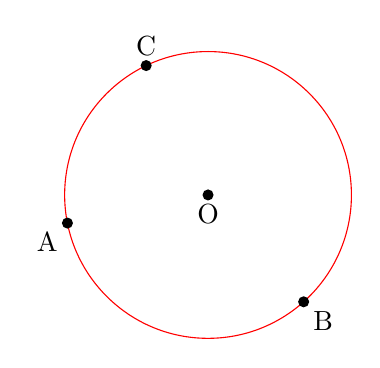
\begin{tikzpicture}
  % 定义三个点的坐标
  \coordinate (A) at (1, 2);
  \coordinate (B) at (4, 1);
  \coordinate (C) at (2, 4);

  % 计算圆心
  \path let
    \p1 = (A), \p2 = (B), \p3 = (C),
    \n{k1} = {(\y2 - \y1) / (\x2 - \x1)},
    \n{k2} = {(\y3 - \y2) / (\x3 - \x2)},
    \n{m1} = {-1 / \n{k1}},
    \n{m2} = {-1 / \n{k2}},
    \n{x} = {(\n{m1} * (\x1 + \x2) / 2 - \n{m2} * (\x2 + \x3) / 2 + (\y2 + \y3) / 2 - (\y1 + \y2) / 2) / (\n{m1} - \n{m2})},
    \n{y} = {\n{m1} * (\n{x} - (\x1 + \x2) / 2) + (\y1 + \y2) / 2}
  in
    coordinate (O) at (\n{x}, \n{y});

  % 计算半径
  \path[draw,red] let
    \p1 = (O), \p2 = (A),
    \n{r} = {sqrt((\x2 - \x1)^2 + (\y2 - \y1)^2)}
  in
    (O) circle (\n{r});

  % 绘制点
  \fill (A) circle (2pt) node[below left] {A};
  \fill (B) circle (2pt) node[below right] {B};
  \fill (C) circle (2pt) node[above] {C};
  \fill (O) circle (2pt) node[below] {O};

\end{tikzpicture}

\end{document}